\documentclass[10pt, regno]{amsart}
\usepackage[utf8]{inputenc}
\usepackage[T1]{fontenc}
\usepackage{amsmath,amssymb}
\usepackage{amsmath}
\usepackage{tikz}
\usetikzlibrary{positioning,matrix,arrows,decorations.pathmorphing, patterns, math, intersections, calc}

\begin{document}

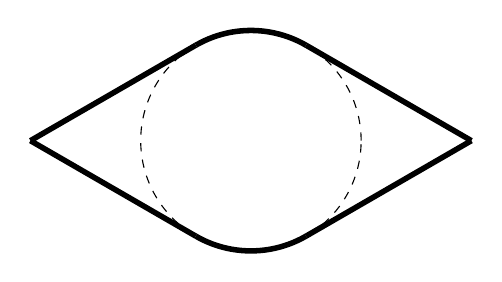
\begin{tikzpicture}[scale=0.7]
\draw [line width=0.4pt,dashed] (0,0) circle (2cm);
\draw [line width=2pt] (-4,0)-- (-1,1.7320508075688774);
\draw [line width=2pt] (1,1.7320508075688772)-- (4,0);
\draw [line width=2pt] (4,0)-- (1,-1.7320508075688774);
\draw [line width=2pt] (-1,-1.7320508075688772)-- (-4,0);
\draw [shift={(0,0)},line width=2pt]  plot[domain=1.0471975511965976:2.0943951023931957,variable=\t]({1*2*cos(\t r)+0*2*sin(\t r)},{0*2*cos(\t r)+1*2*sin(\t r)});
\draw [shift={(0,0)},line width=2pt]  plot[domain=4.1887902047863905:5.235987755982988,variable=\t]({1*2*cos(\t r)+0*2*sin(\t r)},{0*2*cos(\t r)+1*2*sin(\t r)});
\end{tikzpicture}

\end{document}